\documentclass[utf8x, 12pt]{G7-32} 


% --------- -------- SETTINGS --------- --------

% --------- Настройки стиля ГОСТ 7-32 --------

% Гипертекстовое оглавление в PDF
\usepackage[
bookmarks=true, colorlinks=true, unicode=true,
urlcolor=black,linkcolor=black, anchorcolor=black,
citecolor=black, menucolor=black, filecolor=black,
]{hyperref}

\usepackage{graphicx}   % Пакет для включения рисунков
\DeclareGraphicsExtensions{.jpg,.pdf,.png}
\geometry{right=20mm}
\geometry{left=30mm}
\usepackage{enumerate}
\setcounter{tocdepth}{3} % Подробность оглавления


% --------- other settings --------
\usepackage{MnSymbol}
%\usepackage{simpsons}
% --------- -------- SETTINGS --------- --------

% LISTINGS
\usepackage{listings}
\usepackage{color}

\definecolor{dkgreen}{rgb}{0,0.6,0}
\definecolor{gray}{rgb}{0.5,0.5,0.5}
\definecolor{mauve}{rgb}{0.58,0,0.82}

\lstset{frame=tb,
  language=bash,
  aboveskip=3mm,
  belowskip=3mm,
  showstringspaces=false,
  columns=flexible,
  basicstyle={\small\ttfamily},
  numbers=none,
  numberstyle=\tiny\color{gray},
  keywordstyle=\color{blue},
  commentstyle=\color{dkgreen},
  stringstyle=\color{mauve},
  breaklines=true,
  breakatwhitespace=true,
  tabsize=3
}

\begin{document}

\frontmatter 

% --------- -------- TITLE --------- --------

\begin{center} 

\large САНКТ-ПЕТЕРБУРГСИЙ ГОСУДАРСТВЕННЫЙ ПОЛИТЕХНИЧЕСКИЙ УНИВЕРСИТЕТ

\large Кафедра Компьютерных Систем и Программных Технологий \\[5.5cm] 

\huge ОТЧЕТ \\[0.6cm] % название работы, затем отступ 0,6см
\large по лабораторной работе №7\\
\large Тема: <<Сервис тестирования корректности настройки SSL на сервере Qualys SSL Labs --- SSL Server Test>>\\
\large Дисциплина: <<Методы и средства защиты информации>>\\[3.7cm]

\end{center} 

\begin{flushright}
Выполнил: студент гр. 53501/2 \\
Пономарев М.A. \\[1.2cm]


Преподаватель \\
Вылегжанина К.Д.
\end{flushright}


\vfill 

\begin{center} 
\large Санкт-Петербург \\
2015
\end{center} 

\thispagestyle{empty}


% --------- -------- TITLE --------- --------

\thispagestyle{empty}
\setcounter{page}{0}
\tableofcontents
\clearpage
\mainmatter


\chapter{Задание}


\begin{enumerate}
	\item Изучение
	\begin{enumerate}
	\item Изучить лучшие практики по развертыванию SSL/TLS
	\item Изучить основные уязвимости и атаки на SSL последнего времени --- POODLE, HeartBleed
\end{enumerate}
	\item Практическое задание\\
	Выбрать со стартовой страницы SSL Server Test один домен из списка Recent Best и один домен из списка Recent Worst --- изучить отчеты, интерпретировать результаты в разделе Summary
Выбрать для анализа интернет-домен защищенный SSL--шифрованием, проделать следующие шаги:
	\begin{enumerate}
	\item Интерпретировать результаты в разделе Summary
	\item Расшифровать все аббревиатуры шифров в разделе Configuration
	\item Прокомментировать большинство позициq в разделе Protocol Details
	\item Сделать итоговый вывод о реализации SSL на заданном домене
	
\end{enumerate}
\end{enumerate}

Инструмент выполнения:
Qualys SSL Labs --- SSL Server Test


\chapter{Выполнение}

\section{Изучение}

\subsection{Лучшие практики по развертыванию SSL}

\begin{itemize}
	\item Использовать 2048--битные закрытые ключи.
Использовать 2048--битный RSA или 256--битные ECDSA закрытые ключи для всех серверов. Ключи такой крепости безопасны и будут оставаться безопасными в течение значительного периода времени.
	\item Защитить закрытый ключ. Предоставить доступ к ключу как можно меньшей группе сотрудников.
	\item Обеспечить охват всех используемых доменных имен. Убедиться, что сертификаты охватывают все доменные имена, которые используются на сайте.
	\item Приобретать сертификаты у надежного CA.
	\item Использовать надежные алгоритмы подписи сертификата. Безопасность сертификата зависит от длины закрытого ключа и прочности используемой функции хеширования. Сегодня большинство сертификатов используют алгоритм SHA1, который считается слабым. 
	\item Использовать безопасные протоколы. (TLS v1.0/v1.1/v1.2)
	\item Использовать безопасные алгоритмы шифрования. В данном случае подойдут симметричные алгоритмы с ключами более 128 бит.
	\item Контролировать выбор алгоритма шифрования. В SSL версии 3 и более поздних версиях протокола, клиенты отправляют список алгоритмов шифрования, которые они поддерживают, и сервер выбирает один из них для организации безопасного канала связи. Не все сервера могут делать это хорошо, так как некоторые выбирают первый поддерживаемый алгоритм из списка.
	\item Использование Forward Secrecy. Forward Secrecy --- это особенность протокола, который обеспечивает безопасный обмен данными, он не зависит от закрытого ключа сервера. С алгоритмами шифрования, которые не поддерживают Forward Secrecy, возможно расшифровать ранее зашифрованные разговоры с помощью закрытого ключа сервера.
	\item Отключить проверку защищенности по инициативе клиента.
\end{itemize}


\newpage
\subsection{Основные уязвимости и атаки на SSL последнего времени --- POODLE, HeartBleed}

\subsubsection{POODLE}

	POODLE(Padding Oracle On Downgraded Legacy Encryption) --- уязвимость, позволяющая злоумышленнику от имени жертвы отправлять данные на сервер и расшифровывать их если у него есть возможность прослушивать и подменять трафик жертвы. Об уязвимости стало известно после того, как Google опубликовал документ с названием <<This POODLE Bites: Exploiting The SSL 3.0 Fallback>>.

	Уязвимость позволяет злоумышленнику, используя атаку Man--in--the--middle, заставить браузер жертвы использовать SSL 3.0 (более старый протокол) вместо того, чтобы использовать современный TLS, и за счет этого эксплуатировать дыры в безопасности в SSL, чтобы украсть сессии браузера.

	Если и браузер и сервер поддерживают протокол SSL 3.0, атакующий может принудить браузер использовать старый протокол. Другими  словами, хоть и браузер будет пытаться использовать TLS, он будет принужден использовать SSL.


\subsubsection{HeartBleed}
	Heartbleed --- ошибка (переполнение буфера) в криптографическом программном обеспечении OpenSSL, позволяющая несанкционированно читать память на сервере или на клиенте, в том числе для извлечения закрытого ключа сервера. Информация об уязвимости была опубликована в апреле 2014 года, ошибка существовала с конца 2011 года.


\newpage
\section{Практическое задание}

\subsection{Выбрать со стартовой страницы SSL Server Test один домен из списка Recent Best и один домен из списка Recent Worst}


\begin{figure}[hhh!]
	\begin{center}
		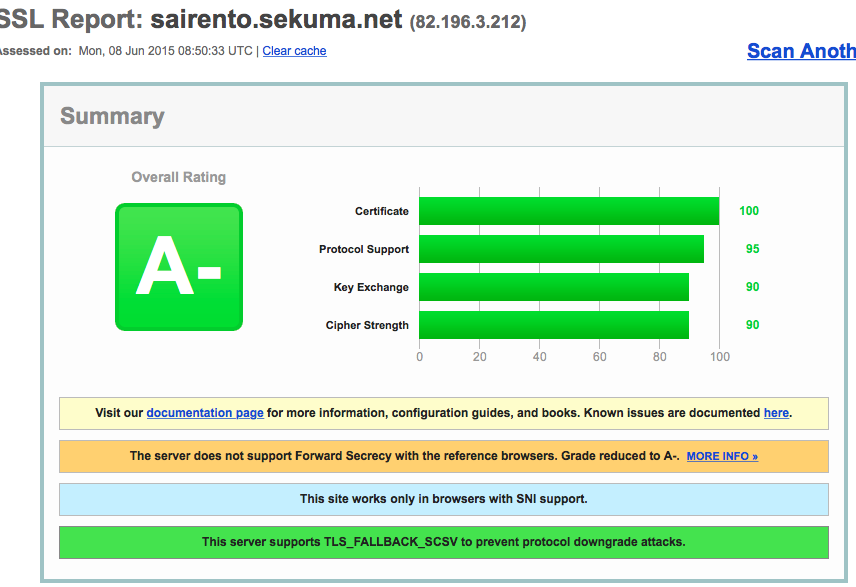
\includegraphics[width=14cm]{img/best}
	\end{center}
	\vspace{-5mm}\caption{Recent best}
\end{figure}


\begin{enumerate}
		\item Сервер не поддерживает поддержку защиты наперед с некоторыми браузерами.
		\item Этот сайт работает только с браузерами с поддержкой SNI(Server Name Indication)
		\item Этот сервер поддерживает TLS\_FALLBACK\_SCSV, чтобы избежать нисходящие атаки
\end{enumerate}


\begin{figure}[hhh!]
	\begin{center}
		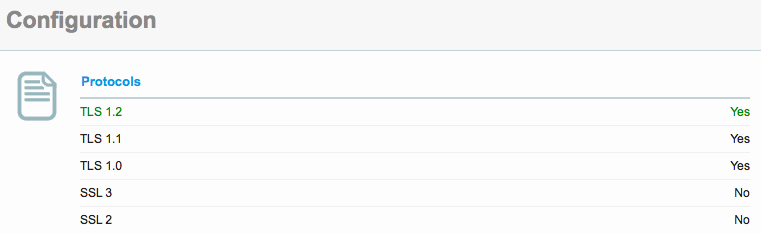
\includegraphics[width=14cm]{img/best2}
	\end{center}
	\vspace{-5mm}\caption{Configuration}
\end{figure}

TLS (Transport Layer Security), как и его предшественник SSL (Secure Sockets Layer) --- криптографические протоколы, обеспечивающие защищённую передачу данных между узлами в сети Интернет. TLS и SSL используют асимметричную криптографию для аутентификации, симметричное шифрование для конфиденциальности и коды аутентичности сообщений для сохранения целостности сообщений.

Данный протокол широко используется в приложениях, работающих с сетью Интернет, таких как веб-браузеры, работа с электронной почтой, обмен мгновенными сообщениями.

Конфигурация поддерживает основные виды TLS, в то же время не поддерживает SSL 3 и SSL 2, что очень хорошо, так как эти протоколы являются устаревшими.


\begin{figure}[hhh!]
	\begin{center}
		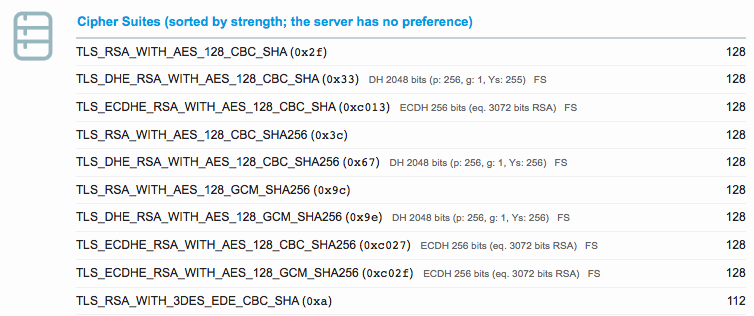
\includegraphics[width=14cm]{img/best3}
	\end{center}
	\vspace{-5mm}\caption{Chiper Suites}
\end{figure}

\begin{itemize}
	\item RSA --- Rivest, Shamir, Adleman  --- криптографический алгоритм
	\item RC4 --- Rivest Chipher 4 --- потоковый шифр 4-й версии
	\item SHA/SHA256/384 --- Secure Hash Algorithm --- алгорим хэширования (цифра соответствует длине ключа)
	\item AES --- Advanced Encryption Standart --- симметричный алгоритм блочного шифрования
	\item GCM и CBC --- два режима блочного шифрования
	\item TLS --- Transport Layer Security --- криптографический протокол
	\item 3DES --- Digital Encryption Standart --- алгоритм блочного шифрования
	\item EDE --- Encrypt, Decrypt, Encrypt --- режим работы алгоритма 3DES
	\item Camalia --- симметричный алгоритм блочного шифрования
\end{itemize}

\newpage


\begin{figure}[hhh!]
	\begin{center}
		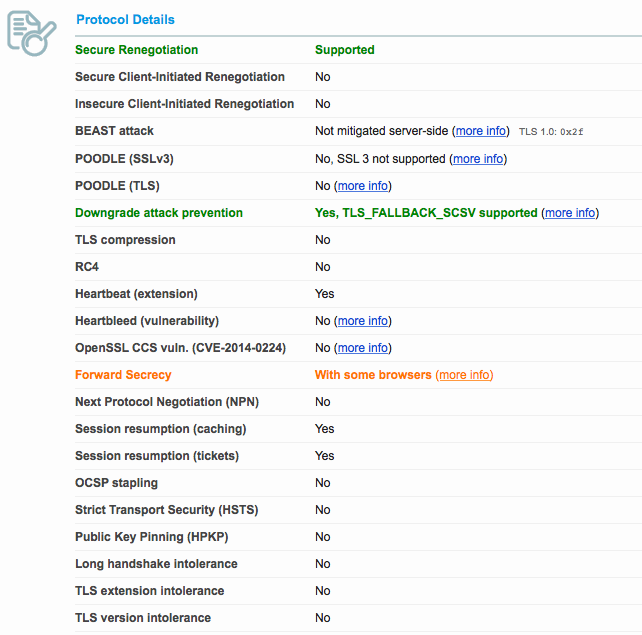
\includegraphics[width=14cm]{img/best4}
	\end{center}
	\vspace{-5mm}\caption{Protocol Details}
\end{figure}

\begin{itemize}
	\item Поддерживает возобновление подключения TLS
	\item Нету поддержки возобновления подключения TLS с инициализированным клиентом. Есть некоторые случаи, в которых возобновление должно быть инициализировано сервером, но нет никакой известной необходимости для клиентов, чтобы это сделать.
	\item BEAST атака смягчена со стороны сервера
	\item Нет POODLE, Heartbleed и RC4 уязвимостей.
	\item OCSP (или Online Certificate Status Protocol) --- протокол, проверяющий, был ли отозван SSL--сертификат. Используя OCSP, браузер посылает запрос к OCSP URL и получает ответ, содержащий состояние достоверности сертификата. Не поддерживается.
\end{itemize}



\newpage

\begin{figure}[hhh!]
	\begin{center}
		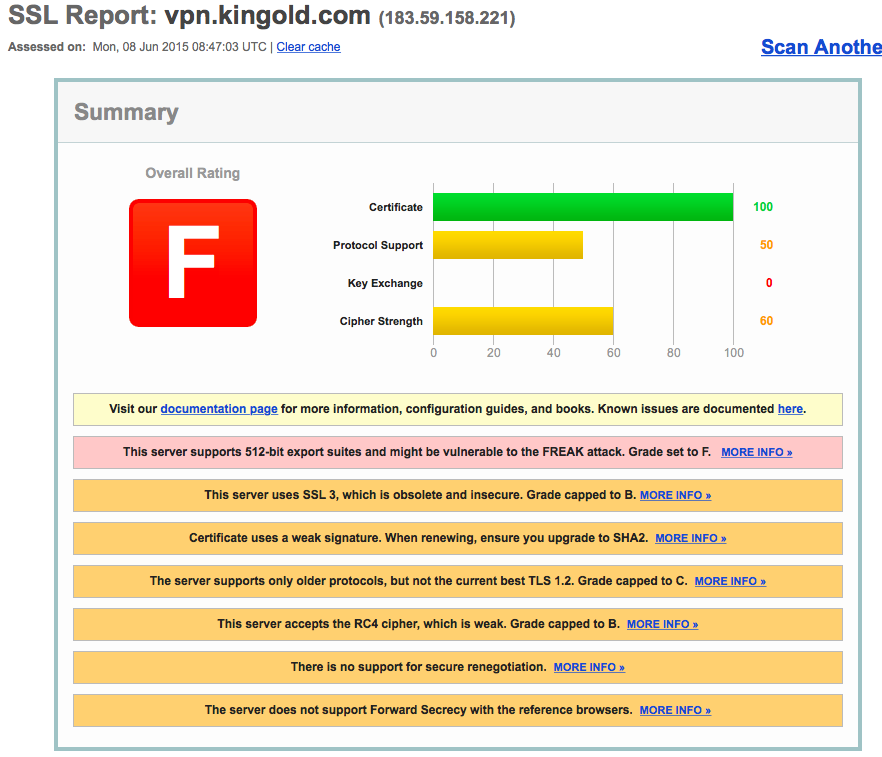
\includegraphics[width=14cm]{img/weak}
	\end{center}
	\vspace{-5mm}\caption{Recent worst}
\end{figure}


\begin{enumerate}
	\item Сервер поддерживает пакеты для экспорта в 512--бит и могут быть уязвимы к FREAK атакам
	\item  Сервер использует устаревший и небезопасный SSL 3 
	\item Сертификат имеет слабую подпись. Использует старый алгоритм шифрования SHA--2
	\item Сервер поддерживает старые протоколы
	\item Использует потоковый шифр RC4, считающийся слабым
	\item Нет поддержки безопасного пересмотра
	\item Сервер не поддерживает поддержку защиты наперед с некоторыми браузерами.
\end{enumerate}

Для более детального описания какой либо информации об уязвимости, на сайте можно нажать вкладку <<MORE INFO>> в соответствующей вкладке.




\section{Сделать итоговый вывод о реализации SSL на заданном домене (для анализа выбран первый)}

В целом, после сервис дает очень развернутую информацию о любом домене, поскольку выбранный для анализа домен был из категории <<A->>, то и критичных уязвимсотей у него не было обнаружено.



\chapter{Выводы}
	В результате выполнения лабораторной работы были изучены возможности веб--сервиса Qalys SSL LABS, который позволяет получить развернутую статистику по уровню защищенности сокетов (SSL) для запрашиваемого домена. 

	Анализируя данные таким способом, можно избавить от дыр в безопасности сервера, закрыв критические уязвимости.
\end{document}
